\documentclass[11pt]{beamer}
\usetheme{default}
\usefonttheme{serif}

\usepackage[utf8]{inputenc}
\usepackage[british]{babel}
\usepackage[T1]{fontenc}
\usepackage{graphicx}
\usepackage{listings}
\usepackage[round, authoryear]{natbib}
\usepackage{booktabs}
\usepackage{amssymb} 

% Pacchetto fondamentale per separare le slide extra dal conteggio totale
\usepackage{appendixnumberbeamer}

% --- Rosso Istituzionale Università di Padova ---
\definecolor{PadovaRed}{HTML}{B20E10} 
\usecolortheme[named=PadovaRed]{structure} 

\setbeamertemplate{caption}[numbered]
\setbeamertemplate{navigation symbols}{} 

% --- FOOTLINE CUSTOM: Pagina X di Y (non conta le pause e si ferma prima dell'appendice) ---
\setbeamertemplate{footline}{%
  \hfill\usebeamerfont{footline}\insertframenumber{} / \insertmainframenumber\hspace*{2ex}\vspace*{1ex}%
}

% --- Informazioni Presentazione ---
\author[Del Col]{Lorenzo Del Col}
\title[Master's Thesis]{The Short, the Long, and the Consequences of VAR Analysis For Structural DSGE Estimation}
\newcommand{\email}{lorenzo.delcol@studenti.unipd.it}

\institute[]{
    \small Supervisor: Professor Efrem Castelnuovo \\
    \vspace{0.3cm}
    \footnotesize \textit{University of Padova} \\ 
    \footnotesize \textit{MSc Applied Economics}
}
\date{July 2026}

\begin{document}

% =======================================
% TITLE
% =======================================

\begin{frame}
\titlepage
\end{frame}

% =======================================
% MOTIVATION
% =======================================

\begin{frame}{Motivation}
    \begin{itemize}
        \item VAR models can be used to estimate DSGE frameworks by IRFs minimization matching
    \end{itemize}
    
    \begin{itemize}  
        \item If the VAR is mispecified the DSGE might also be so
    \end{itemize}
    \vspace{0.1cm}
    \pause
    
    \textbf{Why it is relevant?}
    \begin{itemize}
        \item \textit{``The quality of our strategy (IRFs matching) depends on the \textbf{ability of identified VARs to generate reliable estimates} of the dynamic response of economic variables to shocks.''}
        \vspace{0.1cm}
        \hfill {\small \textbf{\citet{ACEL2011}, p. 3, fn. 10} }
        \pause

        \item \textit{``If the VAR adequately caputeres the DGP, IRFs are optimal at all horizons. 
        \\
        If the \textbf{VAR is mispecified}, however, then the \textbf{specification errors will be computed at each horizon}''}
        \vspace{0.1cm}
        \hfill {\small \textbf{\citet{Ramey2016}, p. 83} }
        \pause
        
        \item VARs and DSGEs are instruments used by central banks to make policy decisions
        \item Misspecification can deliver distorted results mis informing the central banker
    \end{itemize}

\end{frame}

% =======================================
% RESEARCH QUESTION
% =======================================

\begin{frame}{This Paper}\label{slide:this_paper}
    \textbf{Research Question:}
    \begin{itemize}
        \item \textcolor{PadovaRed}{Can VAR truncation bias have significant implications for DSGE estimation?}
    \end{itemize}
    
    \vspace{0.4cm}
    \textbf{What we do:}
    \begin{itemize}
        \item Test if well established facts in the literature are sensitive to the chosen lag structure
    \end{itemize}
    \pause
    
    \vspace{0.4cm}    
    \textbf{Findings:}
    \begin{itemize}
        \item Both VAR based IRFs and structural DSGE parameter estimates are significantly affected by the inclusion of longer lags
    \end{itemize}
    \begin{center}
        \hyperlink{slide:var_irfs}{\beamerbutton{VAR IRFs}} \quad
        \hyperlink{slide:dsge_irfs}{\beamerbutton{DSGE IRFs}} \quad
        \hyperlink{slide:dsge_params}{\beamerbutton{DSGE Parameters}}
    \end{center}
\end{frame}

% =======================================
% RELATED LITERATURE
% =======================================

\begin{frame}{Related Literature}
    \textbf{IRFs:}
    \begin{itemize}
        \item \citep{Moller_Wolf2021, Ludwig2026}
    \end{itemize}
    \textbf{DSGE IRFs matching with VARs}
    \begin{itemize}
        \item \citep{CEE2005, ACEL2011, Jarocinski_Karadi2020}
    \end{itemize}
    \textbf{Truncation Bias}
    \begin{itemize}
        \item \citep{Long_Lag2025, Baumeister2025}
    \end{itemize}
    \textbf{Long Lag VARs}
    \begin{itemize}
        \item \citep{Antolin-Diaz_Surico2025}
    \end{itemize}
\end{frame}

% =======================================
% ILLUSTRATION OF TRUNCATION BIAS PROBLEM
% =======================================

\begin{frame}{Illustration of Truncation Bias Problem}
    \begin{equation}
        Y_t = B_1Y_{t-1} + \cdots + B_pY_{t-p} + u_t, \qquad E(u_t u_t') = \Sigma
    \end{equation}

    \begin{equation}
        B(L) = B_1L + \cdots + B_pL^p
    \end{equation}

    \begin{itemize}
        \item The VAR with $p < p^{*}$ suffers from truncation bias.\footnote{Where $p^{*}$ denotes the DGP true lag length.}

        \item Lag truncation biases the reduced form coefficients $B(L)$ and the reduced form variance covariance matrix $\Sigma$, which are the two main ingredients for IRF estimation.
    \end{itemize}

    \begin{equation}
        \mathrm{IRF} = f\bigl(B(L),\Sigma\bigr)
    \end{equation}
\end{frame}

% =======================================
% LONG LAG 1
% =======================================

\begin{frame}{Long-Lag}
    \citet{Long_Lag2025} argue that increasing the lag structure improves IRFs estimates obtaining:
    \pause
    \vspace{0.4cm}
    
    \textbf{Lower Bias}
    \begin{itemize}
        \item By reducing the truncation bias misspecification
    \end{itemize}
    \pause

    \vspace{0.4cm}
    \textbf{Lower Variance}
    \begin{itemize}
        \item Misspecification reduction lowers the variance of the residuals
        \item This variance reduction counteracts the imprecision caused by increased parametrisation
    \end{itemize}
\end{frame}

% =======================================
% LONG LAG 2
% =======================================

\begin{frame}{Long-Lag}
    \begin{figure}
        \centering
        \IfFileExists{../../Output/VAR_Residuals_RMSE_Estimates/InSample_Residuals_Fed_Funds_Rate.pdf}
            {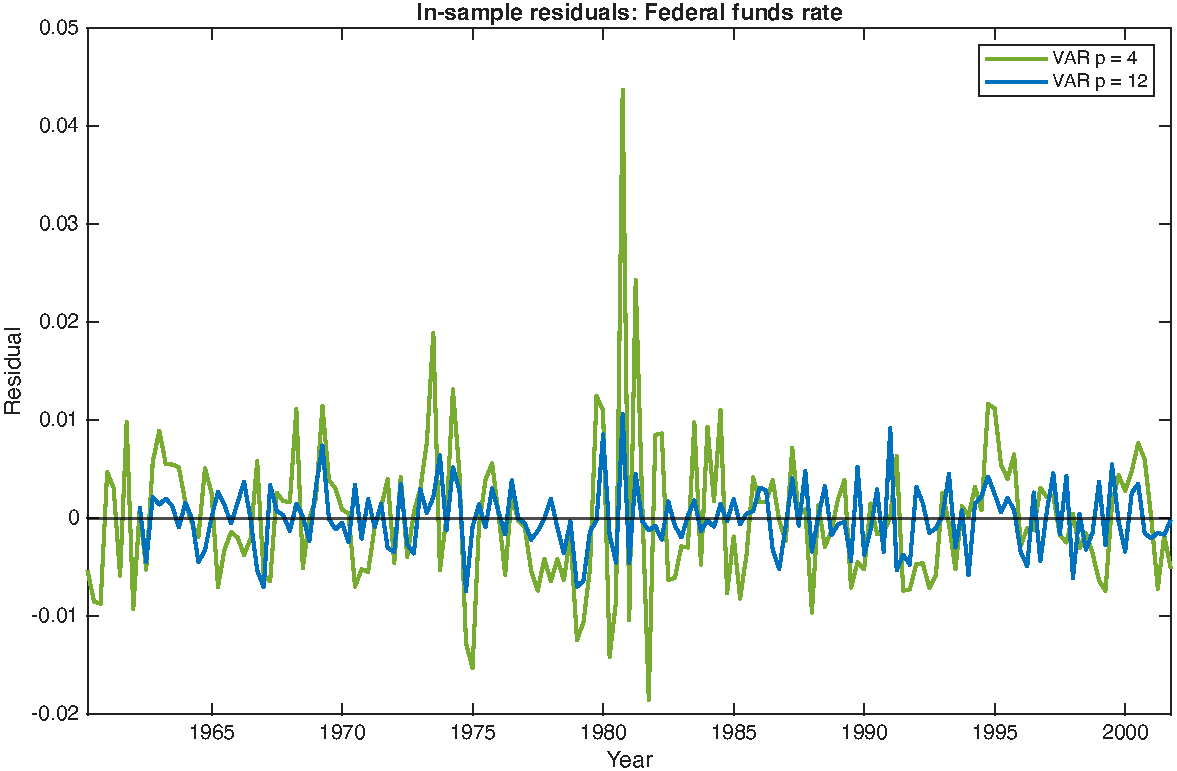
\includegraphics[width=0.95\linewidth]{../../Output/VAR_Residuals_RMSE_Estimates/InSample_Residuals_Fed_Funds_Rate.pdf}}
            {\fbox{Missing file: InSample\_Residuals\_Fed\_Funds\_Rate.pdf}}
        \caption{FFR Residuals Comparison Across lag 4 Vs 12 }
        \label{fig:placeholder1}
    \end{figure}
\end{frame}

% =======================================
% LONG LAG BENEFITS
% =======================================

\begin{frame}{Long-Lag Benefits}
    The variance-reducing effect of lower misspecification often dominates the penalty of increased parameterisation.
    \vspace{0.4cm}
    
    Compared to short-lag VARs, Long-Lag VARs have:
    \begin{itemize}
        \item Reduced truncation bias
        \item More precise inference
        \item Lower MSE
        \item Better coverage
    \end{itemize}
\end{frame}

% =======================================
% BASELINE EXERCISE
% =======================================

\begin{frame}{Baseline Exercise}
    Framework:
    \begin{itemize}
        \item \textbf{\citet{ACEL2011}}'s DSGE\footnote{Where the replication package provided by the authors refers to the 2005 NBER working paper}
        \item Sample period 1959:Q2-2001:Q4
    \end{itemize}
    
    Exercise:
    \begin{itemize}
        \item We re-estimate the VAR with different lag order
        \item Re-estimate the DSGE by IRFs matching
        \item Analyse possible variations in the structural parameters across different lag choice
        \item Search for possible drivers of structural changes
    \end{itemize}
\end{frame}

% =======================================
% ACEL2011'S MECHANISM 1
% =======================================

\begin{frame}{ACEL2011's Mechanism}
    Classic NK models accountes for inflation inertia by assuming that firms re-optimise their prices every six quarter or even less often
    \begin{itemize}
        \item \citet{ACEL2011}'s model inflation is inertial despite firms re-optimise prices average every 1.5 quarters
        \item Inertia is explained by the fact that, when firms re optimise they do it by a small amount because each firm's short run marginal cost is increasing in its own output
        \item The key assumption is that, in any given period a firm's capital stock is pre-determined and is firm specific
    \end{itemize}

    \vspace{0.5cm}
    They create a two model that builds on \citet{CEE2005}: 
    \begin{itemize}
        \item Capital is Homogeneous
        \item Capital Firm-Specific
    \end{itemize}
\end{frame}

% =======================================
% ACEL2011'S MECHANISM 2
% =======================================

\begin{frame}{ACEL2011's Mechanism (Cond't)}
\begin{itemize}
    \item When log-linearized, the only difference in characterizing equilibrium equations lies in the Phillips Curve equation
\end{itemize}

\begin{align}
    \Delta\hat{\pi}_t &= \mathbb{E} [\beta\Delta\hat{\pi}_{t+1} + \gamma\hat{s}_t|\Omega_t] 
    \label{eq:Phillips_Curve}
    \\
    \gamma &= \frac{(1-\xi_p)(1-\beta\xi_p)}{\xi_p}\chi 
    \label{eq:Phillips_Curve_Slope}
\end{align}

\begin{itemize}
    \item The $s_t$ are the economy-wide marginal costs, $\gamma$ is the Phillips' Curve slope and $\xi_p$ is the Calvo's price stickyness parameter
    \item $\chi$ reduces the sensitivity of inflation to marginal costs in the firm specific capital model
    \item The two models are observationally equivalent in terms of prices and quantities, the difference between the two models lies in the $\gamma$, not on $\xi_p$
\end{itemize}
\end{frame}

% =======================================
% ACEL2011'S MECHANISM 3
% =======================================

\begin{frame}{ACEL2011's Mechanism (Cond't)}
\begin{itemize}
    \item In the \textbf{Homogeneous} capital model $\gamma$ (eq. \ref{eq:Phillips_Curve_Slope}) depends on agent's discount rate $\beta$ and on the fraction $1 -\xi_p$ of firms that can optimise within the quarter
    \item In the \textbf{Firm Specific} $\gamma$ depends on a broader sets of structural parameters, is a non linear function with a non trivial representation.
    \item The more costly is for a firm to vary capital utilization, the steeper is its marginal cost curve and hence the smaller $\gamma$ is
    \item The more elastic is the individual firm's demand curve, the smaller is $\gamma$
\end{itemize}
\end{frame}

% =======================================
% ACEL2011'S RESULTS
% =======================================

\begin{frame}{ACEL2011 Results}
    The estimated $\gamma$ is 0.0402, this implies that in:
    \begin{itemize}
        \item Homogeneous Capital model, firms change prices every 5.6 quarters, with an implied $\xi_p = 0.82 $
        \item Firms Specific model, firms change prices every 1.5 quarters, with an implied $\xi_p = 0.33 $
    \end{itemize}
The reason why the models have such different implications for firms' pricing behaviour is that, firm's demand curve are highly elastic and their marginal curves are very steep
\\
Only the Firm-specific capital model reconcile the micro-macro pricing conflict
\vspace{0.5cm}
\pause

\begin{itemize}
    \item \textbf{Are these results robust to an enriched lag structure of the VAR?}
\end{itemize}
\end{frame}

% =======================================
% VAR IRFs MP
% =======================================

\begin{frame}{VAR IRFs; Monetary Policy Shock}\label{slide:var_irfs}
    \begin{figure}
        \centering
        \IfFileExists{../../Output/VAR_IRFs_Long_Lag_CI_PE_4_8_12_Plots/Monetary_Policy_Shock/Comparison_Lags_4_8_12.pdf}
            {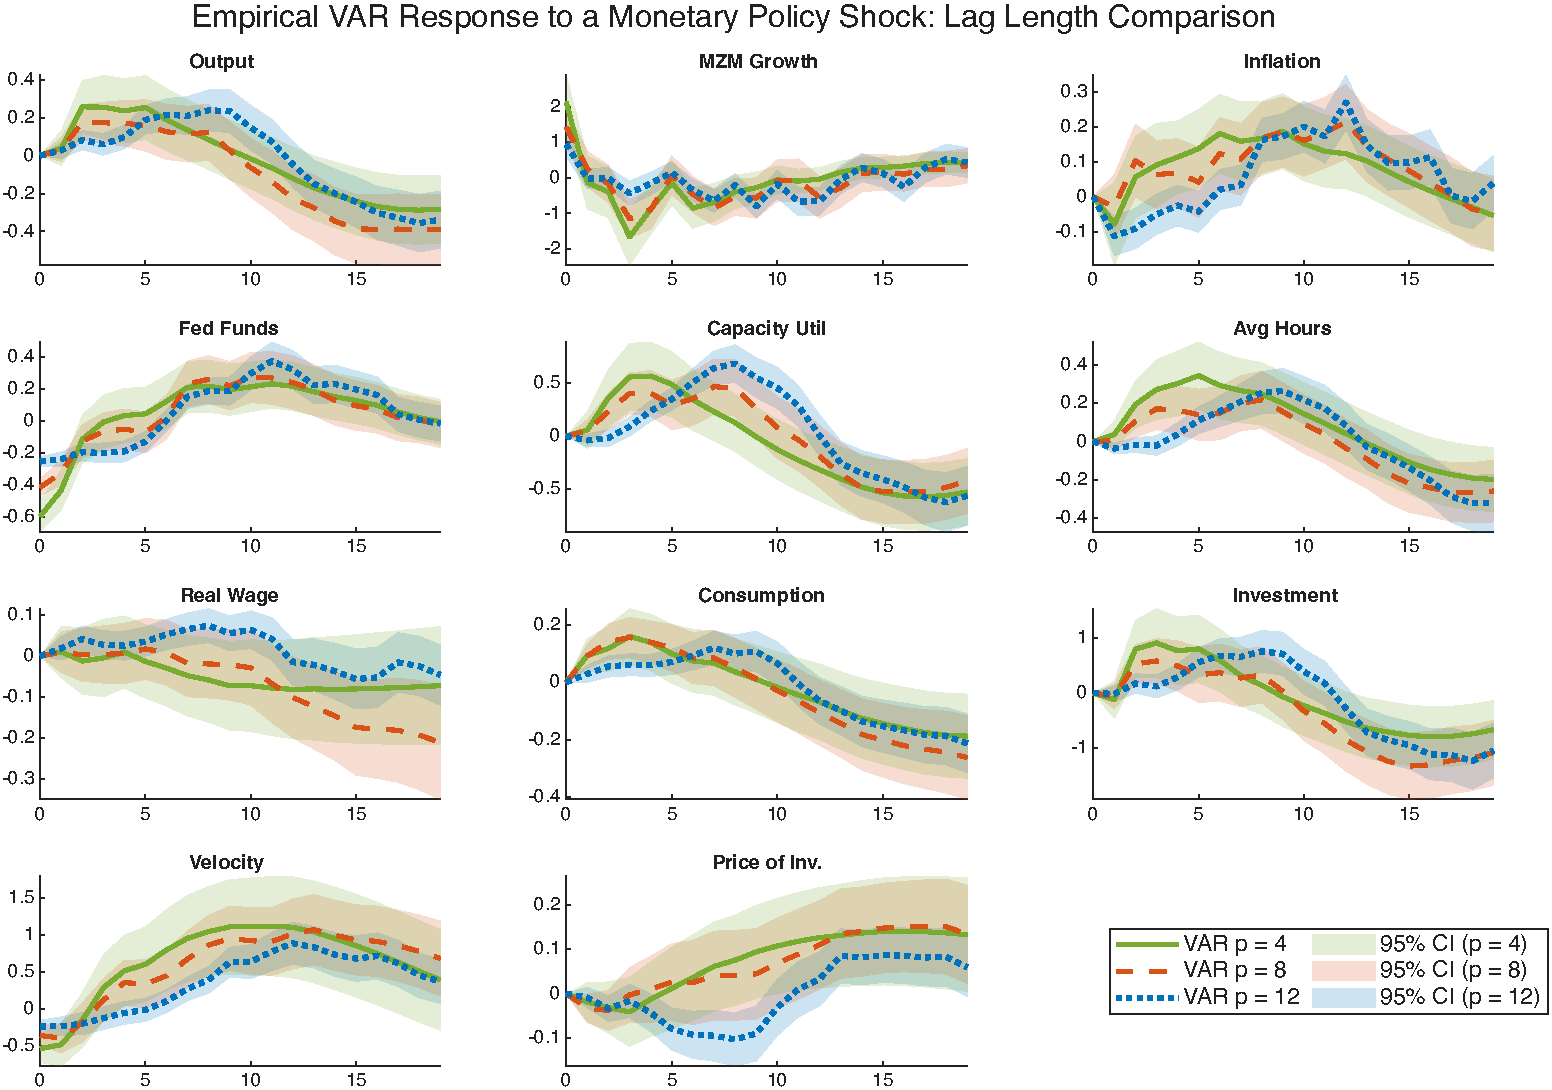
\includegraphics[width=0.95\linewidth]{../../Output/VAR_IRFs_Long_Lag_CI_PE_4_8_12_Plots/Monetary_Policy_Shock/Comparison_Lags_4_8_12.pdf}}
            {\fbox{Missing file: Comparison\_Lags\_4\_8\_12.pdf}}
        \caption{IRFs VAR Comparison: Monetary Policy Shock}
        \label{fig:placeholder2}
    \end{figure}
    \begin{flushright}
        \hyperlink{slide:this_paper}{\beamerreturnbutton{Back}}
    \end{flushright}
\end{frame}

% =======================================
% DSGE IRFs MP
% =======================================

\begin{frame}{DSGE IRFs; Monetary Policy Shock}\label{slide:dsge_irfs}
    \begin{figure}
        \centering
        \IfFileExists{../../Output/DSGE_IRFs_Long_Lag_Comparison_4_8_12_Plots/Monetary_Policy_Shock/DSGE_Comparison_Lags_4_8_12.pdf}
            {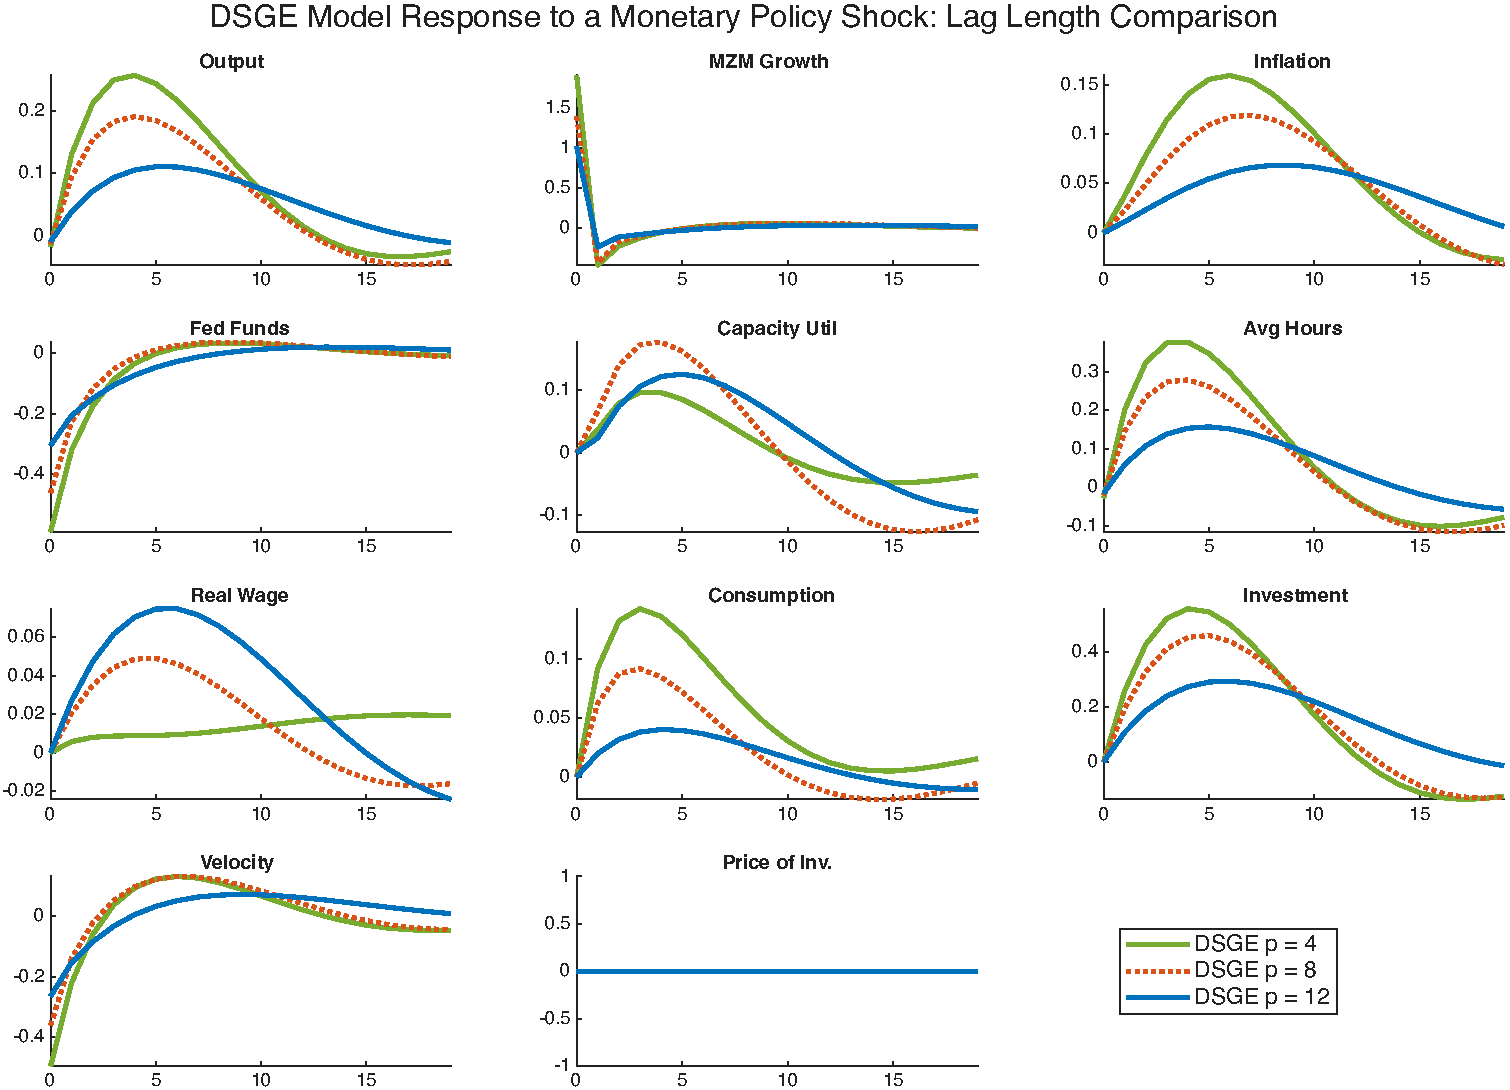
\includegraphics[width=0.95\linewidth]{../../Output/DSGE_IRFs_Long_Lag_Comparison_4_8_12_Plots/Monetary_Policy_Shock/DSGE_Comparison_Lags_4_8_12.pdf}}
            {\fbox{Missing file: DSGE\_Comparison\_Lags\_4\_8\_12.pdf}}
        \caption{IRFs DSGE Comparison: Monetary Policy Shock}
        \label{fig:placeholder3}
    \end{figure}
    \begin{flushright}
        \hyperlink{slide:this_paper}{\beamerreturnbutton{Back}}
    \end{flushright}
\end{frame}

% =======================================
% DSGE PATAMETERS TABLE 4 8 12
% =======================================

\begin{frame}{DSGE Structural Parameters}\label{slide:dsge_params}
\IfFileExists{../../Output/DSGE_Parameters_Comparison/dsge_params_table_beamer_4_8_12.tex}
    {\begin{table}[htpb]
    \centering
    \scriptsize
    \begin{tabular}{lccc}
    \toprule
    \textbf{Parameter} & \textbf{VAR $p=4$} & \textbf{VAR $p=8$} & \textbf{VAR $p=12$} \\
    \midrule \multicolumn{4}{c}{\textit{Structural Estimated Frictions}} \\
    Price markup ($\lambda_f$) & 1.0100 & 1.0100 & 1.0100 \\
    & (-) & (-) & (-) \\
    Wage stickiness ($\xi_w$) & 0.7221*** & 0.5617*** & 0.4838*** \\
    & (0.1506) & (0.1142) & (0.0757) \\
    Phillips curve slope ($\gamma$) & 0.0402 & 0.0402 & 0.0129*** \\
    & (0.0246) & (0.0598) & (0.0042) \\
    Capacity util. cost ($\sigma_a$) & 1.9938 & 0.1175 & 0.0042 \\
    & (2.6066) & (0.6299) & (0.0230) \\
    Habit formation ($b$) & 0.7066*** & 0.6935*** & 0.8596*** \\
    & (0.0463) & (0.0570) & (0.0203) \\
    Inv. adj. cost ($S^{\prime\prime}$) & 3.2807* & 3.0372* & 6.8431*** \\
    & (1.8874) & (1.5506) & (2.3306) \\
    Money demand elast. ($\epsilon$) & 0.8077*** & 0.7531*** & 0.8346*** \\
    & (0.2111) & (0.1473) & (0.1944) \\
    \midrule \multicolumn{4}{c}{\textit{Implied Price Stickiness}} \\
    Homogeneous capital ($\xi_{p, hom}$) & 0.8213 & 0.8213 & 0.8958 \\
    & (-) & (-) & (-) \\
    Firm-specific capital ($\xi_{p, fs}$) & 0.3372 & 0.6448 & 0.8884 \\
    & (-) & (-) & (-) \\
    \bottomrule
    \end{tabular}
\end{table}
}
    {\fbox{Missing file: dsge\_params\_table\_beamer\_4\_8\_12.tex}}
    \begin{flushright}
        \hyperlink{slide:this_paper}{\beamerreturnbutton{Back}}
    \end{flushright}
\end{frame}

% =======================================
% IMPLIED AVERAGE TIME TABLE 4 8 12
% =======================================

\begin{frame}{Implied Average Time between Re-Optimization}
\IfFileExists{../../Output/DSGE_Parameters_Comparison/implied_duration_A4_4_8_12.tex}
    {\begin{table}[htpb]
    \centering
    \small
    \renewcommand{\arraystretch}{1.2}
    \caption{Implied Average Time between Re-Optimization}
    \label{tab:implied_duration_4_8_12}
    \begin{tabular}{lccc}
        \toprule
        \textbf{Model Specification} & \textbf{VAR $p=4$} & \textbf{VAR $p=8$} & \textbf{VAR $p=12$} \\
        \midrule

        \multicolumn{4}{l}{\textit{Homogeneous Capital Model}} \\
        Calvo parameter ($\xi_{p, hom}$) & 0.82 & 0.82 & 0.90 \\
        Implied duration (quarters)      & \textbf{5.6} & \textbf{5.6} & \textbf{9.6} \\

        \midrule
        \multicolumn{4}{l}{\textit{Firm-Specific Capital Model}} \\
        Calvo parameter ($\xi_{p, fs}$) & 0.34 & 0.64 & 0.89 \\
        Implied duration (quarters)     & \textbf{1.5} & \textbf{2.8} & \textbf{9.0} \\

        \bottomrule
    \end{tabular}

    \vspace{0.2cm}
    \raggedright
    \scriptsize{\textit{Note:} Implied duration is calculated as $D = 1/(1 - \xi_p)$.}
\end{table}
}
    {\noindent\fbox{Image Path Broken or File Missing}}
\end{frame}


% =======================================
%  NEXT STEPS
% =======================================

\begin{frame}{Next Step}
    In the ACEL2011 exercise
    \begin{itemize}
        \item MonteCalvo of the Phillipcs curve slope components to simulate the Calvo Price Parametes' Standard Error
        \item Check the estimated parameters likelihood function
        \item Leverage on Canova's tip; long-lag VARs mess up HD
        \item Long-Lag VARs are a good aproximation of Trend-Cycle VARs, are we specifying better the trend?
        \item Make sure the VARs starts from the same point in time, we need to drop the first 12 data points fro each VAR for comparison pourposes
    \end{itemize}
\end{frame}

\begin{frame}
\begin{center}
    \Large Thanks a lot for your attention! \\
    \vspace{1cm}
    \normalsize \email
\end{center}
\end{frame}

% =========================================================
% APPENDICE
% =========================================================
\appendix

\begin{frame}{VAR IRFs; Monetary Policy Shock}
\begin{figure}
    \centering
    \IfFileExists{../../Output/VAR_IRFs_Long_Lag_CI_PE_4_8_12_Plots/Monetary_Policy_Shock/Comparison_Lags_4_8_12.pdf}
        {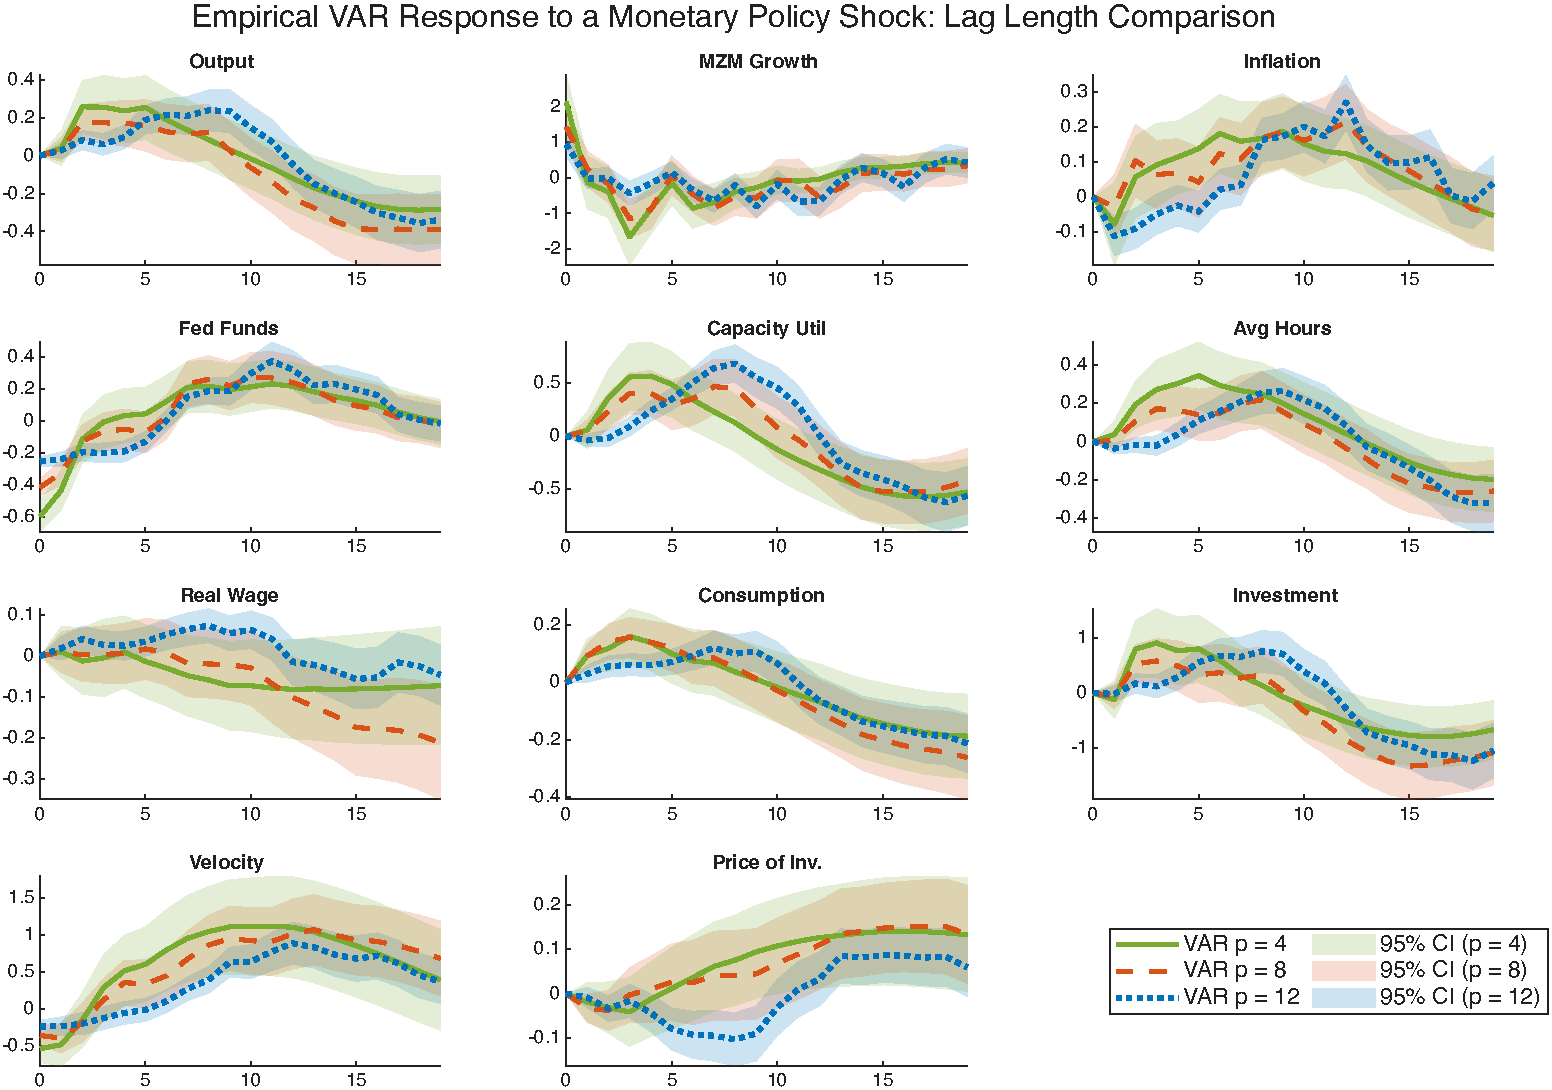
\includegraphics[width=0.95\linewidth]{../../Output/VAR_IRFs_Long_Lag_CI_PE_4_8_12_Plots/Monetary_Policy_Shock/Comparison_Lags_4_8_12.pdf}}
        {\fbox{Missing file: Comparison\_Lags\_4\_8\_12.pdf}}
    \caption{IRFs VARs all CI Comparison: Monetary Policy Shock}
    \label{fig:placeholder4}
\end{figure}
\end{frame}

% =========================================================
% TRUCCO PER NASCONDERE LA BIBLIOGRAFIA
\setbox0=\vbox{
\begin{minipage}{\textwidth}
    \bibliographystyle{apalike}
    \bibliography{biblio}
\end{minipage}
}

% =========================================================
% BIBLIOGRAFIA
%\begin{frame}[allowframebreaks]{References}
%    \bibliographystyle{plainnat}
%    \bibliography{biblio}
%\end{frame}

\end{document}